\chapter{Qiskit}\label{ch:qiskit}
This chapter describes the Qiskit library and slightly touches on other solutions that can be used to program quantum computers.
The 7-year work of IBM culminated in the middle of February 2024, when they released version 1.0.0.

Before we dive into benchmarking our ansatzes we need to make clear a few terms.
\begin{definition} (Shots) 
    A shot is a single run of a quantum circuit. As we know from the previous chapters, the quantum computation is probabilistic. The results of individual shots can be different. The more shots we run, the more accurate the results are.
\end{definition}

In the below picture, we can see a distribution of measurements when using different numbers of shots. Each one of the states is equally likely. With an increasing number of shots, we can observe that the distribution converges to a uniform distribution.

\begin{figure}[H]
    \centering
    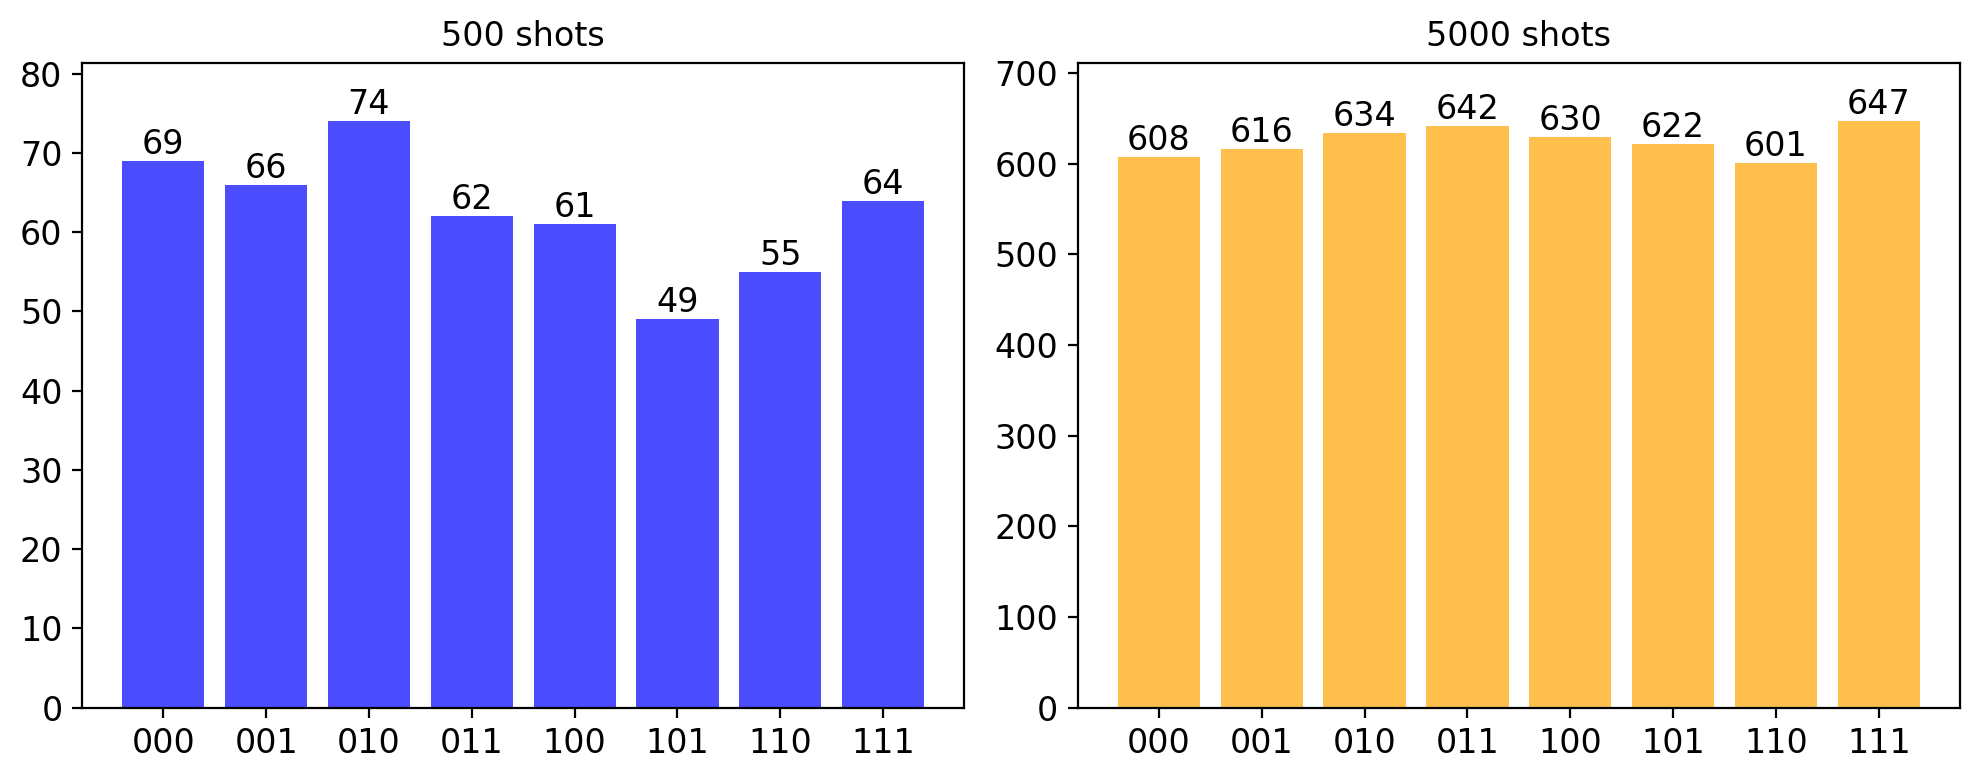
\includegraphics[width=\linewidth]{shots-distribution.png}
    \caption{Measurement distribution for different numbers of shots.}\label{fig:output}
\end{figure}

\begin{definition} (Iteration) 
    An iteration is a single run of the VQE, thus run a quantum circuit to find an expectation value of the Hamiltonian and then use the classical optimizer to find the best parameters for the next iteration.
\end{definition}

\begin{definition}(Function evaluation)
    Our cost function is passed to a classical optimizer which tries to determine the best parameters that can lead to minimal value. Function evaluations are a number of how many times the cost function was evaluated. Therefore in a single iteration can optimizer evaluate the cost function multiple times.
\end{definition}

\todo{Programing of quantum computers is like assembly}
\todo{HarTree jednotky}
\todo{Initial point}
\todo{Hyperparameters}
\todo{("fault-tolerant QPUs") FTQC vs NISQ}
\todo{UCC vs HEA https://arxiv.org/pdf/2310.02511.pdf}
\todo{Divide shots into stages}
\todo{communtative hamiltonian}
